\chapter[Merkezi Limit Teoremi ve Standart Hata]{Merkezi Limit Teoremi ve Standart Hata; MLT'nin İstatistiksel Çıkarımdaki Rolü}
\label{ch:clt-se}

\begin{prismbox}[PrismLight]{Öğrenme çıktıları}
Bu bölümün sonunda:
\begin{itemize}
  \item bireysel standart puan ile standartlaştırılmış örneklem ortalamasını ayırabilecek,
  \item Merkezi Limit Teoreminin ne söylediğini ve ne söylemediğini açıklayabilecek,
  \item standart hatayı hesaplayıp örneklem hacmiyle ilişkisini yorumlayabilecek,
  \item normal yaklaşımın uygunluğunu veri yapısına göre değerlendirebileceksiniz.
\end{itemize}
\end{prismbox}

\begin{prerequisitebox}
Örnekleme dağılımı, örneklem ortalaması, varyans ve karekök işlemi
bilinmelidir. Normal dağılımın simetrik yapısı hakkında temel farkındalık
yeterlidir.
\end{prerequisitebox}

Bu bölüm, Bölüm~\ref{sec:sampling-distribution}'de kurulan örnekleme dağılımı
fikrini normal yaklaşım ve standart hata hesabına taşır.

\section{Normal dağılım ve standartlaştırma}

Normal dağılım $\mu$ çevresinde simetrik, çan biçimli sürekli bir dağılımdır.
Bir $x$ değerinin merkezden kaç standart sapma uzakta olduğunu gösteren
standart puan
\[
z=\frac{x-\mu}{\sigma}
\]
biçimindedir. Standartlaştırma, farklı ölçeklerdeki değerleri ortak bir
ölçekte karşılaştırmayı sağlar.

Örneklem ortalaması standartlaştırılırken paydada bireysel standart sapma
değil, ortalamanın standart hatası kullanılır:
\[
Z=\frac{\bar X-\mu}{\sigma/\sqrt n}.
\]
İlk formül tek bir gözlemin konumunu, ikinci formül ise bir örneklem
ortalamasının beklenen merkezden uzaklığını ölçer.

\section{Merkezi Limit Teoremi}
\label{sec:clt}

Bağımsız, aynı dağılımlı ve sonlu varyanslı gözlemlerde örneklem hacmi
arttıkça
\[
\frac{\bar X-\mu}{\sigma/\sqrt n}
\]
istatistiğinin dağılımı yaklaşık standart normal dağılıma yaklaşır. MLT ham
verinin normal olduğunu değil, örneklem ortalamasının uygun biçimde
standartlaştırılmış örnekleme dağılımının normale yaklaştığını söyler.

Evren normal dağılıyorsa $\bar X$ her $n$ için tam olarak normaldir. Evren
normal değilse MLT yaklaşık bir sonuç verir ve yaklaşım genellikle $n$
büyüdükçe iyileşir. Yaklaşımın hızı evren dağılımına bağlıdır: simetrik ve
hafif kuyruklu dağılımlarda daha hızlı, çok çarpık veya ağır kuyruklu
dağılımlarda daha yavaş olabilir \citep{hogg2015,akdeniz1998,erbas2011}.

\begin{figure}[H]
\centering
\begin{tikzpicture}[x=0.42cm,y=0.45cm]
  \foreach \shift/\label in {0/{$n=1$},3.8/{$n=5$},7.6/{$n=30$}} {
    \begin{scope}[xshift=\shift cm]
      \draw[->,PrismGray] (0,0)--(6.8,0);
      \node[below,font=\scriptsize] at (3.4,-0.15) {\label};
    \end{scope}
  }
  \foreach \x/\h in {0.5/5,1.5/3.3,2.5/2.2,3.5/1.4,4.5/0.8,5.5/0.4}
    \fill[PrismWarnOrange!80!black] (\x-0.35,0) rectangle (\x+0.35,\h);
  \begin{scope}[xshift=3.8cm]
    \foreach \x/\h in {0.5/0.8,1.5/2.0,2.5/3.4,3.5/3.7,4.5/2.4,5.5/1.0}
      \fill[PrismSubheadingBlue!70] (\x-0.35,0) rectangle (\x+0.35,\h);
  \end{scope}
  \begin{scope}[xshift=7.6cm]
    \foreach \x/\h in {0.5/0.4,1.5/1.3,2.5/3.2,3.5/4.8,4.5/3.2,5.5/1.3,6.5/0.4}
      \fill[PrismBlue!78] (\x-0.35,0) rectangle (\x+0.35,\h);
  \end{scope}
\end{tikzpicture}
\caption{Çarpık bir evrende örneklem ortalamasının dağılımının şematik değişimi.}
\label{fig:clt-progression}
\end{figure}

Şekil~\ref{fig:clt-progression}, MLT'nin ham dağılımı değil örneklem
ortalamasının dağılımını dönüştürdüğünü görsel olarak özetler.

\section{Standart hata}
\label{sec:standard-error}

Standart hata, bir tahmin edicinin örnekleme dağılımındaki standart sapmadır.
Ortalama için
\[
\SE(\bar X)=\frac{\sigma}{\sqrt n}
\]
olur. Evren standart sapması bilinmediğinde uygulamada
$\SE(\bar X)\approx s/\sqrt n$ kullanılır.

Standart hata gözlenmiş bir örneklem için belirsizlik tahminidir. Örneklem
standart sapması $s$, bilinmeyen $\sigma$ yerine kullanıldığında ek belirsizlik
oluşur. Ortalama çıkarımında özellikle küçük örneklemlerde normal dağılım
yerine Student $t$ dağılımının kullanılmasının nedeni budur.

\begin{mistakebox}
Standart sapma bireysel gözlemlerin yayılımını, standart hata ise bir
tahminin örneklemden örnekleme değişkenliğini ölçer.
\end{mistakebox}

\section{Karekök yasası ve çıkarım}

Standart hata $1/\sqrt n$ oranında azalır. Belirsizliği yaklaşık yarıya
indirmek için örneklem hacmini dört katına çıkarmak gerekir. MLT ve standart
hata birlikte, tahminlerin çevresinde güven aralığı kurulmasına ve test
istatistiklerinin referans dağılımlarla karşılaştırılmasına temel sağlar.

\begin{table}[H]
\centering
\caption{$\sigma=20$ için örneklem hacmi ve standart hata.}
\label{tab:se-by-n}
\begin{tabular}{rrrr}
\toprule
$n$ & $\sqrt n$ & $\SE(\bar X)$ & Önceki satıra göre değişim \\
\midrule
25  & 5  & 4 & --- \\
100 & 10 & 2 & yarıya iner \\
400 & 20 & 1 & yeniden yarıya iner \\
\bottomrule
\end{tabular}
\end{table}

Tablo~\ref{tab:se-by-n}'de görüldüğü gibi örneklem hacmini iki katına çıkarmak
standart hatayı yarıya indirmez;
$1/\sqrt2\approx0{,}707$ katına indirir. Bu azalan getiri, örneklem planında
hassasiyet ile maliyet arasında denge kurulmasını gerektirir.

\section{Çözümlü örnek: örneklem hacminin etkisi}

Bir başarı testinin standart sapması yaklaşık 12 puan olsun. $n=36$ için
\[
\SE(\bar X)=\frac{12}{\sqrt{36}}=2
\]
puan, $n=144$ için ise $\SE(\bar X)=1$ puandır. Standart hatayı yarıya
indirmek için örneklem hacmi dört katına çıkarılmıştır. Bu sonuç daha büyük
örneklemin bireysel puanları birbirine yaklaştırdığını değil, ortalama
tahminini daha kararlı hâle getirdiğini gösterir.

\section{MLT ne zaman dikkatle kullanılmalıdır?}
\label{sec:clt-cautions}

``$n\geq30$ ise her zaman normal yaklaşım kullanılabilir'' evrensel bir kural
değildir. Gerekli örneklem hacmi evren dağılımının çarpıklığına, kuyruklarına
ve aykırı değerlerine bağlıdır. Çok çarpık veya ağır kuyruklu dağılımlarda
daha büyük örneklem gerekebilir. Bağımlı gözlemler ve sistematik örnekleme
hataları da MLT tarafından düzeltilmez.

Örneklem oranı için normal yaklaşımın uygunluğu yalnız toplam $n$ ile değil,
beklenen başarı ve başarısızlık sayılarıyla değerlendirilir. Yaygın bir ön
kontrol $np$ ve $n(1-p)$ değerlerinin yeterince büyük olmasıdır. $p$ sıfıra
veya bire çok yakınsa büyük sayılabilecek bir örneklemde bile yaklaşım zayıf
kalabilir.

\begin{sezgibox}
MLT bir veri temizleme veya örnekleme kalitesi teoremi değildir. Uygun
koşullarda bir istatistiğin örnekleme dağılımını yaklaşık normal bir referansla
karşılaştırabilmemizi sağlar.
\end{sezgibox}

\section{Çarpık evrenden benzetim}

Üstel dağılım belirgin biçimde sağa çarpıktır. Aşağıdaki kod, $n=1$, $5$ ve
$30$ için örneklem ortalamalarının dağılımını karşılaştırır. Tüm panellerin
merkezi aynı hedefe yaklaşırken dağılım daralır ve daha simetrik görünür.

\begin{softwarebox}
\begin{lstlisting}
import numpy as np
import matplotlib.pyplot as plt

rng = np.random.default_rng(2026)
fig, axes = plt.subplots(1, 3, figsize=(9, 3))

for ax, n in zip(axes, [1, 5, 30]):
    means = rng.exponential(scale=10,
                            size=(10000, n)).mean(axis=1)
    ax.hist(means, bins=35, density=True,
            color="#8FB8D8", edgecolor="white")
    ax.axvline(10, color="#1F4E79", linewidth=2)
    ax.set_title(f"n = {n}")

plt.tight_layout()
plt.show()
\end{lstlisting}
Grafikler karşılaştırılırken yalnız biçime değil, yatay eksenin ölçeğine ve
dağılımın genişliğine de bakılmalıdır.
\end{softwarebox}

\section{Çıkarım için karar zinciri}

\begin{enumerate}
  \item Gözlemlerin hangi tasarımla üretildiğini ve bağımsızlığın makul olup olmadığını belirleyin.
  \item Ham dağılımı çarpıklık, aykırı değer ve veri sınırları bakımından inceleyin.
  \item İlgilenilen istatistiğin standart hatasını uygun formülle hesaplayın.
  \item Normal veya $t$ yaklaşımının gerekçesini belirtin.
  \item Güven aralığı ya da test sonucunu bağlam ve varsayımlarla birlikte yorumlayın.
\end{enumerate}

\begin{assumptionbox}
MLT'nin temel biçimi bağımsız, aynı dağılımlı ve sonlu varyanslı gözlemleri
varsayar. Kümeleşme, zaman bağımlılığı veya aşırı ağır kuyruklar varsa
$\sigma/\sqrt n$ formülü ve normal yaklaşım doğrudan kullanılamayabilir.
\end{assumptionbox}

\section{Çözümlü problemler}

\subsection*{Problem 1: Bireysel z-puanı ile ortalamanın standartlaştırılması}

Bir başarı puanı evreninde $\mu=50$ ve $\sigma=10$ olsun. Tek bir öğrencinin
puanı 65'tir. Ayrıca $n=25$ öğrencilik bir sınıfın ortalaması 54 bulunmuştur.
Bireysel puanı ve sınıf ortalamasını standartlaştırarak sonuçları yorumlayın.

\textbf{Çözüm.} Tek bir öğrencinin puanı için bireysel standart sapma
kullanılır:
\[
z=\frac{65-50}{10}=1{,}50.
\]
Öğrencinin puanı evren ortalamasının 1,5 standart sapma üzerindedir. Sınıf
ortalaması için önce standart hata hesaplanır:
\[
\SE(\bar X)=\frac{10}{\sqrt{25}}=2.
\]
Ardından örneklem ortalaması
\[
Z=\frac{54-50}{2}=2
\]
olarak standartlaştırılır. Sınıf ortalaması beklenen evren ortalamasının iki
standart hata üzerindedir.

İki standartlaştırmanın payları ve yorumları farklıdır. İlk değer bir
öğrencinin diğer bireylere göre konumunu, ikinci değer ise bir sınıf
ortalamasının tekrarlı örnekleme altında beklenen merkezden uzaklığını
gösterir.

\begin{mistakebox}
Sınıf ortalamasını standartlaştırırken paydada doğrudan $\sigma=10$
kullanmak $Z=0{,}4$ sonucunu verir ve örneklem ortalamasının daha düşük
değişkenliğini göz ardı eder. Ortalama için doğru ölçek $\sigma/\sqrt n$'dir.
\end{mistakebox}

\subsection*{Problem 2: MLT ile örneklem ortalaması olasılığı}

Bir sınav puanı evreninin ortalaması 80, standart sapması 15'tir. Dağılım tam
olarak normal olmayabilir. Rastgele ve bağımsız $n=100$ öğrencilik bir
örneklem için $\P(\bar X>83)$ olasılığını yaklaşık olarak bulun.

\textbf{Çözüm.} Örneklem hacmi büyük olduğundan, dağılım aşırı ağır kuyruklu
değilse MLT örneklem ortalamasına normal yaklaşım sağlar. Standart hata
\[
\SE(\bar X)=\frac{15}{\sqrt{100}}=1{,}5
\]
ve sınır değerin standartlaştırılmış karşılığı
\[
Z=\frac{83-80}{1{,}5}=2
\]
olur. Standart normal dağılım tablosundan
\[
\P(\bar X>83)\approx\P(Z>2)=1-0{,}9772=0{,}0228.
\]
Dolayısıyla aynı evrenden seçilen 100 kişilik örneklemlerin yaklaşık yüzde
2,28'inde ortalamanın 83'ü aşması beklenir.

\textbf{Yorum.} Bu hesap tek bir öğrencinin 83'ten yüksek puan alma
olasılığı değildir. İlgilenilen rassal nicelik 100 öğrencinin ortalamasıdır.

\subsection*{Problem 3: Çarpık evrende örneklem hacminin rolü}

Bekleme süresi dağılımı belirgin biçimde sağa çarpık, ortalaması 10 dakika ve
standart sapması 10 dakika olsun. $n=4$ ve $n=100$ için örneklem ortalamasının
merkezini, standart hatasını ve beklenen biçimini karşılaştırın.

\textbf{Çözüm.} Her iki örneklem hacminde de örneklem ortalamasının beklenen
değeri 10 dakikadır. Standart hatalar
\[
SE_{n=4}=\frac{10}{\sqrt4}=5,
\qquad
SE_{n=100}=\frac{10}{\sqrt{100}}=1
\]
olarak bulunur. Büyük örneklemde ortalamalar 10 çevresinde çok daha dar bir
aralıkta toplanır.

$n=4$ için örnekleme dağılımı evrendeki güçlü sağ çarpıklığın önemli bir
bölümünü koruyabilir; normal yaklaşım otomatik olarak güvenilir değildir.
$n=100$ için MLT etkisi daha güçlüdür ve örneklem ortalamasının dağılımı
genellikle daha simetrik, çan biçimine daha yakın görünür. Bununla birlikte
bağımsızlık ve sonlu varyans koşulları yine gereklidir.

\textbf{Raporlama örneği.} ``Bekleme sürelerinin ham dağılımı sağa çarpık
olmasına rağmen 100 gözlemli örneklem ortalamasının dağılımı MLT uyarınca
yaklaşık normal ve standart hatası 1 dakika olarak değerlendirildi.''

\subsection*{Problem 4: Hedef standart hataya göre örneklem hacmi}

Bir ölçeğin evren standart sapmasının yaklaşık 18 puan olduğu bilinmektedir.
Ortalama tahmininin standart hatasının en fazla 1,5 puan olması isteniyor.
Bağımsız basit rastgele örnekleme altında gerekli en küçük örneklem hacmini
bulun.

\textbf{Çözüm.} Hedef
\[
\frac{\sigma}{\sqrt n}\leq1{,}5
\]
eşitsizliğidir. $\sigma=18$ yazılırsa
\[
\frac{18}{\sqrt n}\leq1{,}5,
\qquad
\sqrt n\geq\frac{18}{1{,}5}=12,
\qquad n\geq144
\]
elde edilir. En az 144 bağımsız gözlem gerekir.

Bu hesap yalnız örnekleme değişkenliğine dayalı bir başlangıç planıdır.
Yanıtlamama, küme örneklemesi, alt grup analizleri veya beklenenden yüksek
değişkenlik söz konusuysa hedeflenen başlangıç örneklemi artırılmalıdır.

\subsection*{Problem 5: Oran için normal yaklaşımın denetlenmesi}

Nadir görülen bir eğitim desteğinden yararlanma oranının $p=0{,}02$ olduğu
varsayılsın. $n=200$ ve $n=1000$ için beklenen başarı ve başarısızlık
sayılarını hesaplayın; normal yaklaşımın uygunluğunu karşılaştırın.

\textbf{Çözüm.} $n=200$ için
\[
np=200(0{,}02)=4,
\qquad n(1-p)=200(0{,}98)=196.
\]
Beklenen başarı sayısı yalnız 4'tür. Yaygın ön koşullardan biri olan her iki
beklenen sayının en az 10 olması sağlanmadığı için $\hat p$ için normal
yaklaşım zayıf olabilir.

$n=1000$ için
\[
np=1000(0{,}02)=20,
\qquad n(1-p)=1000(0{,}98)=980
\]
olur. Her iki sayı da yeterince büyük olduğundan normal yaklaşım çok daha
makuldür. Burada yalnız toplam örneklem hacmine bakmak yeterli değildir;
oranın sıfıra yakınlığı, etkili başarı sayısını küçük tutmaktadır.

\begin{outputguidebox}
Normal yaklaşım kullanan bir yazılım çıktısında yalnız toplam $n$ değerini
değil, ham dağılımın biçimini, aykırı değerleri, bağımsızlık varsayımını ve
oran analizlerinde başarı--başarısızlık sayılarını kontrol edin. Yazılımın
sonuç üretmesi yaklaşımın uygun olduğunu kanıtlamaz.
\end{outputguidebox}

\section{Literatür verisiyle yazılım uygulamaları}
\label{sec:spss-b05}

\textbf{Amaç ve veri.} \texttt{b05.csv} aynı 2.000 tekrarda 5, 30 ve
100 gözlemli ortalamaları içerir \citep{cortez2008data}.
Kaynak notların tamamı bir benzetim dağılımı kabul edilerek standart sapma
$N$ böleniyle $\sigma_{\rm amp}=\SPEmpSigma$ hesaplanmıştır.
Standartlaştırmada $(\bar x-\mu_{\rm amp})/(\sigma_{\rm amp}/\sqrt n)$ kullanılır.


\textbf{Ortak veri.} Doğrulanan B05 uygulamasında üç yazılım da
\nolinkurl{companion/spss/csv/b05.csv} dosyasındaki hazır tekrarları
kullanmıştır. Dosya 2.000 satır ve yedi sütun içerir. B04'ten farklı
olarak 100 çekimlik ortalamalar ve standartlaştırılmış değerler de vardır;
B04 dosyasını yeniden adlandırmak yeterli değildir. Bu karşılaştırma
Excel içe aktarmanın doğrulandığı anlamına gelmez. Kodları
\texttt{companion} klasörünü içeren paket kökünden çalıştırın;
veri sözlüğü için bkz. sayfa~\pageref{sec:spss-guide}.

\subsection{IBM SPSS uygulaması}
\textbf{Başlamadan önce.} Aşağıdaki komut dosyası B05 CSV verisini
açar ve analiz eder. Menü yolunu kullanacaksanız önce veri açma ve
tanımlama komutlarını \texttt{EXECUTE} satırı dahil çalıştırın.

\begin{spssadimlar}
\spssadim{\emph{Analyze $\to$ Descriptive Statistics $\to$ Descriptives} yolunda \texttt{ort5}, \texttt{ort30}, \texttt{ort100}, \texttt{z100} seçin; \emph{Options} altında ortalama ve standart sapmayı isteyip çalıştırın.}
\spssadim{\emph{Graphs $\to$ Legacy Dialogs $\to$ Histogram} yolunda önce \texttt{z5}, sonra \texttt{z100} için ayrı histogramlar alın; normal eğriyi ekleyin.}
\spssadim{\emph{Transform $\to$ Compute Variable} yolunu açın. \emph{Target Variable} alanına \texttt{kapsama} yazın.}
\spssadim{\emph{Numeric Expression} alanına \texttt{ABS(z100)<=1.96} yazıp \emph{OK} seçin. Bu gösterge, aralık içinde kalan tekrarları 1 ile kodlar.}
\spssadim{\emph{Analyze $\to$ Descriptive Statistics $\to$ Frequencies} yolunda \texttt{kapsama} için tablo alın. 1 kategorisinin yüzdesini okuyun; payda 2.000 benzetim tekrarıdır.}
\end{spssadimlar}

{\raggedright
\noindent\textbf{Komutların görevi.} \texttt{COMPUTE} kapsama göstergesini oluşturur; \texttt{FREQUENCIES} yüzdesini verir. \texttt{GRAPH} önceden hesaplanmış standartlaştırılmış ortalamaları gösterir.\par}

\textbf{Uygulama kodu:} \texttt{b05}. Doğrulanan veri dosyası
\texttt{companion/spss} altındaki \texttt{csv/b05.csv} dosyasıdır.

\begin{lstlisting}[style=prismSPSS]
SET DECIMAL=DOT.
GET DATA /TYPE=TXT
 /FILE='companion/spss/csv/b05.csv'
 /ENCODING='UTF8'
 /ARRANGEMENT=DELIMITED /DELCASE=LINE
 /DELIMITERS="," /QUALIFIER='"'
 /FIRSTCASE=2
 /VARIABLES=rep F8.0
 ort5 F20.12 z5 F20.12 ort30 F20.12 z30 F20.12
 ort100 F20.12 z100 F20.12.
FILTER OFF.
WEIGHT OFF.
SPLIT FILE OFF.
VARIABLE LABELS
 rep 'Benzetim tekrar numarasi'
 ort5 '5 cekimin ortalamasi'
 ort30 '30 cekimin ortalamasi'
 ort100 '100 cekimin ortalamasi'
 z5 'Standartlastirilmis 5 cekim ortalamasi'
 z30 'Standartlastirilmis 30 cekim ortalamasi'
 z100 'Standartlastirilmis 100 cekim ortalamasi'.
VARIABLE LEVEL rep (NOMINAL)
 ort5 ort30 ort100 z5 z30 z100 (SCALE).
FORMATS ort5 ort30 ort100 z5 z30 z100 (F12.9).
EXECUTE.
DESCRIPTIVES VARIABLES=ort5 ort30 ort100 z100
 /STATISTICS=MEAN STDDEV.
GRAPH /HISTOGRAM(NORMAL)=z5.
GRAPH /HISTOGRAM(NORMAL)=z100.
COMPUTE kapsama=(ABS(z100)<=1.96).
VALUE LABELS kapsama
 0 'Aralik disinda' 1 'Aralik icinde'.
VARIABLE LEVEL kapsama (NOMINAL).
FORMATS kapsama (F1.0).
FREQUENCIES VARIABLES=kapsama.
\end{lstlisting}

\begin{outputguidebox}
\textbf{Paylaşılan SPSS çıktısıyla doğrulanan değerler.}
$n=5,30,100$ için kuramsal standart hatalar sırasıyla
\SPTheoryFiveSE, \SPTheoryThirtySE\ ve \SPTheoryHundredSE;
benzetimdeki standart sapmalar ise \SPSimFiveSD, \SPSimThirtySD\ ve
\SPSimHundredSD\ bulunmuştur. Kuramsal değerler kaynak dağılımdan
hesaplanır; sonlu tekrar sayısı küçük farklar doğurur.
\texttt{z100} standart sapması \SPSimZSD\ ile 1'e yakındır.
\texttt{kapsama}=1 yüzdesi \SPSimCoverage'tır: standartlaştırılmış
ortalamaların yaklaşık yüzde 95'i $[-1{,}96;1{,}96]$ aralığındadır.
Bu oran gerçek bir hedef evren için genelleme garantisi değildir.
\end{outputguidebox}


\par\noindent\begin{minipage}{\linewidth}
\subsection{R uygulaması}
\label{sec:r-gercek-b05}

\texttt{abs(z100)<=1.96} göstergesinin ortalaması benzetimdeki kapsama oranıdır. Grafik üzerindeki eğri standart normal referanstır.

\begin{lstlisting}[style=prismR]
d <- read.csv("companion/spss/csv/b05.csv")
stopifnot(!anyNA(d))
print(sapply(d[c("ort5", "ort30", "ort100", "z5", "z100")],
  function(degerler) c(n=length(degerler),
    mean=mean(degerler), sd=sd(degerler))))
kapsama <- abs(d$z100) <= 1.96
print(table(kapsama))
print(100 * mean(kapsama))
par(mfrow=c(1, 2))
for (v in c("z5", "z100")) {
  hist(d[[v]], breaks=seq(-5, 5, by=.25),
       probability=TRUE, main=v, xlab=v,
       xlim=c(-5, 5), ylim=c(0, .6))
  curve(dnorm(x), add=TRUE, col="blue")
  abline(v=c(-1.96, 1.96), lty=2)
}
par(mfrow=c(1, 1))
\end{lstlisting}

\textbf{Çıktıyı okuma.} Paylaşılan R çıktısı 2.000 satır, yedi sütun
ve her sütunda sıfır eksik değer gösterir. Beş değişkenin \texttt{n},
\texttt{mean} ve \texttt{sd} satırları doğrulanmıştır. Buradaki
\texttt{n}, çekim sayısı değil tekrar sayısıdır. \texttt{TRUE}, kapsama
tablosundaki ``Aralık içinde'' kategorisine karşılık gelir.
\end{minipage}\par

\par\noindent\begin{minipage}{\linewidth}
\subsection{Python uygulaması}
\label{sec:python-b05}

Mantıksal göstergenin ortalaması kapsama oranını verir. \texttt{stats.norm.pdf} standart normal yoğunluğu çizer.

\begin{lstlisting}[style=prismPythonApp]
import pandas as pd
import numpy as np
from scipy import stats
import matplotlib.pyplot as plt

d = pd.read_csv("companion/spss/csv/b05.csv")
assert not d.isna().any().any()
print(d[["ort5", "ort30", "ort100", "z5", "z100"]].agg(
    ["count", "mean", "std"]))
kapsama = d.z100.abs() <= 1.96
print(kapsama.value_counts().sort_index())
print(100*kapsama.mean())
fig, axes = plt.subplots(1, 2)
for ax, v in zip(axes, ["z5", "z100"]):
    ax.hist(d[v], bins=np.linspace(-5, 5, 41), density=True)
    grid = np.linspace(-5, 5, 1000)
    ax.plot(grid, stats.norm.pdf(grid)); ax.set_title(v)
    ax.set_xlim(-5, 5); ax.set_ylim(0, .6)
    for sinir in [-1.96, 1.96]:
        ax.axvline(sinir, linestyle="--", color="gray")
plt.tight_layout(); plt.show()
\end{lstlisting}

\textbf{Çıktıyı okuma.} Paylaşılan Python çıktısı da 2.000 satır,
yedi sütun ve her sütunda sıfır eksik değer gösterir. \texttt{count},
R'deki \texttt{n}; \texttt{std} ise \texttt{sd} satırıdır. Kapsama
frekansları ve yüzdeleri R ve SPSS ile eşleşir. Bu uygulama bir hipotez
testi veya $p$ değeri üretmez.
\end{minipage}\par

\subsection{Sonuçların karşılaştırılması ve ortak rapor}
12 Eylül 2026'da paylaşılan SPSS tabloları ve histogramları, R ve Python
metin çıktıları ve grafikleriyle karşılaştırılmıştır. Beş değişkenin
tekrar sayısı, ortalaması ve standart sapmasından oluşan 15 hücre,
R ve Python'da gösterilen bilimsel gösterim hassasiyetinde eşleşmiştir.
Bu değerler proje CSV'sinden yapılan hesaplarla da uyumludur. SPSS
tablosundaki dört değişkenin özetleri ve \texttt{z5} histogramında
gösterilen özetler, gösterildikleri yuvarlama hassasiyetinde uyumludur.
Aşağıdaki tablolar çıktıların kitap düzenine uyarlanmış özetidir;
ekran görüntüsü değildir.

\begin{table}[H]
\centering
\caption{B05 tekrar ortalamalarının ve standartlaştırılmış değerlerin özetleri}
\label{tab:b05-dogrulanmis-betimsel}
\begin{tabular}{@{}lrrr@{}}
\toprule
Değişken & Tekrar sayısı & Ortalama & Std. sapma \\
\midrule
\texttt{ort5} & 2.000 & 10,367800 & 2,078856 \\
\texttt{ort30} & 2.000 & 10,419050 & 0,844512 \\
\texttt{ort100} & 2.000 & 10,415250 & 0,458914 \\
\texttt{z5} & 2.000 & $-0{,}023159$ & 1,015916 \\
\texttt{z100} & 2.000 & 0,000131 & 1,002951 \\
\bottomrule
\end{tabular}
\par\smallskip
{\footnotesize Ortalamalar ve standart sapmalar altı ondalık basamağa
yuvarlanmıştır. Standart sapmalar, tekrarlar üzerinden 1.999 böleniyle
hesaplanmıştır; standartlaştırmada kullanılan kaynak dağılımın
$\sigma_{\rm amp}$ değeriyle karıştırılmamalıdır.\par}
\end{table}

\begin{table}[H]
\centering
\caption{B05'te $|z_{100}|\leq 1{,}96$ koşulunun doğrulanmış frekansları}
\label{tab:b05-dogrulanmis-kapsama}
\begin{tabular}{@{}lrr@{}}
\toprule
Kategori & Frekans & Yüzde \\
\midrule
Aralık dışında & 108 & 5,4 \\
Aralık içinde & 1.892 & 94,6 \\
Toplam & 2.000 & 100,0 \\
\bottomrule
\end{tabular}
\par\smallskip
{\footnotesize Kapsama göstergesinde eksik değer yoktur. SPSS'in
\emph{Percent} ve \emph{Valid Percent} sütunları eşittir;
yüzdelerin paydası 2.000 tekrardır.\par}
\end{table}

\begin{figure}[H]
\centering
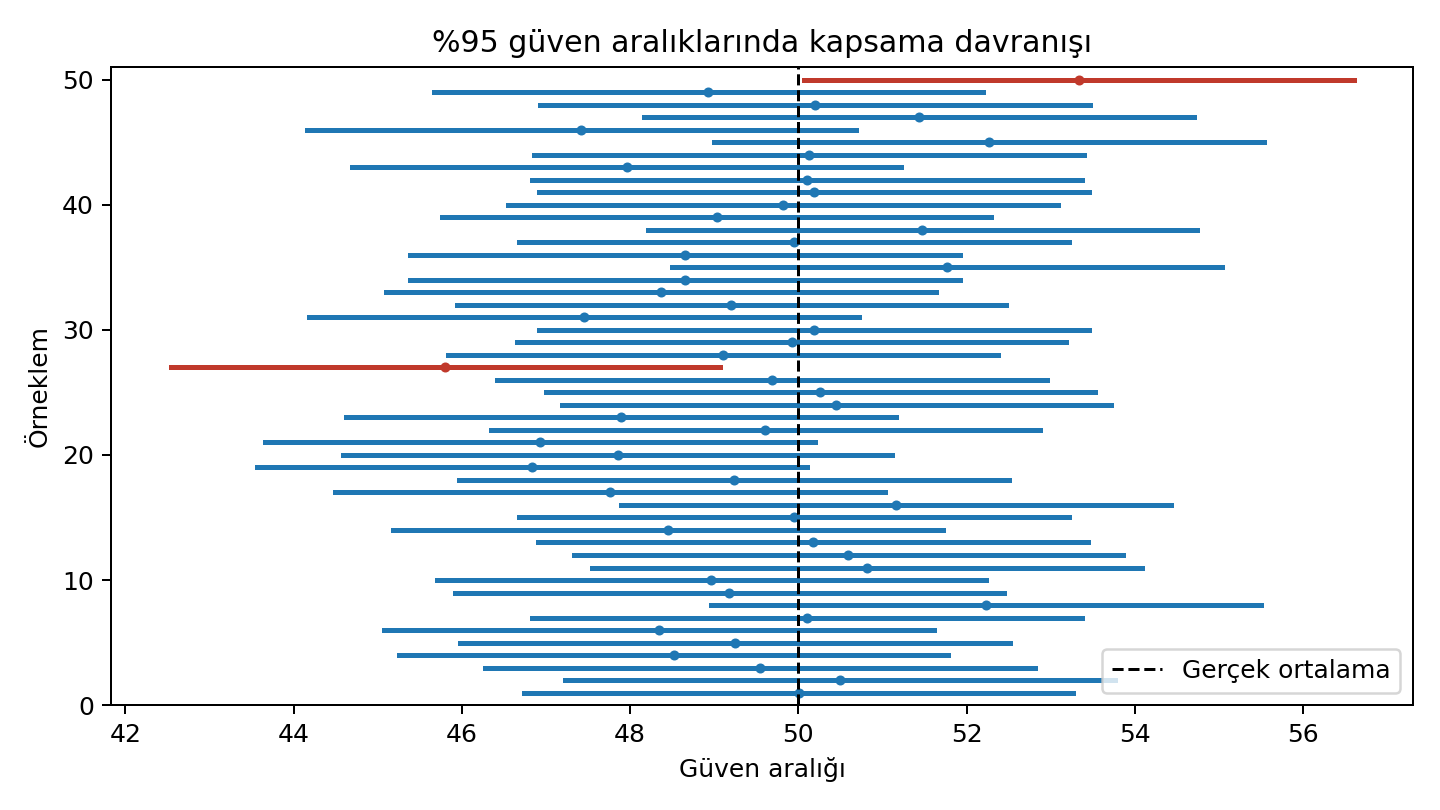
\includegraphics[width=\linewidth]{assets/ch03-kapsama.png}
\caption{B05 için paylaşılan Python histogramları. Kırmızı eğri standart
normal yoğunluğu, kesikli çizgiler $-1{,}96$ ve $+1{,}96$ sınırlarını
gösterir. İki panelde eksen ölçekleri ortaktır.}
\label{fig:b05-dogrulanmis-grafikler}
\end{figure}

\Needspace{19\baselineskip}
\begin{outputguidebox}
Tablo~\ref{tab:b05-dogrulanmis-betimsel} içinde çekim sayısı 5'ten
100'e çıkarken ortalamaların standart sapması 2,078856'dan 0,458914'e
iner. Standartlaştırılmış \texttt{z5} ve \texttt{z100} değerlerinin
standart sapmaları ise 1'e yakındır. Bu nedenle
Şekil~\ref{fig:b05-dogrulanmis-grafikler}, ham ortalamaların daralmasını
değil, standartlaştırılmış dağılımların biçimini karşılaştırır.

Tablo~\ref{tab:b05-dogrulanmis-kapsama} içindeki \%94,6, 1.892 tekrarın
$|z_{100}|\leq1{,}96$ koşulunu sağlamasıdır. Eşdeğer olarak,
$\bar{x}_{100}\pm1{,}96\sigma_{\rm amp}/\sqrt{100}$ aralıklarının
1.892'si benzetimde kullanılan $\mu_{\rm amp}$ değerini kapsar.
Bu, bireysel notların yüzde 94,6'sını kapsayan bir aralık değildir.

R ve Python grafikleri standart normal referans kullanır; SPSS
histogramındaki eğri ise gösterilen değişkenin ortalama ve standart
sapmasına uydurulmuştur. SPSS frekans, R ve Python yoğunluk ölçeği
kullanır; histogramların birebir aynı görünmesi beklenmez. Görsel uyum
normalliği kanıtlamaz. Hazır tekrarlar yeniden üretilmemiştir;
aynı tekrardaki farklı büyüklükteki ortalamalar ortak çekimler içerir.
Hesaplama uyumu, kaynak öğrenci verisinin temsil gücünü kanıtlamaz.
\end{outputguidebox}

\textbf{Raporlama örneği (doğrulanmış çıktılarla).}
``Ampirik not dağılımına dayalı 2.000 tekrarda, 100 çekimlik
ortalamaların ortalaması 10,415250 ve standart sapması 0,458914
bulunmuştur. Kuramsal standart hata yaklaşık \SPTheoryHundredSE'tir.
Standartlaştırılmış ortalamaların ortalaması 0,000131, standart sapması
1,002951'dir. Tekrarların 1.892'si (\%94,6) belirtilen kapsama koşulunu
sağlamıştır. Sonuçlar benzetim dağılımına ilişkindir; gerçek bir hedef
evren için kapsama veya genelleme garantisi olarak yorumlanmamıştır.''


\textbf{Görev.} Örneklem hacmini dört katına çıkarmanın standart hatayı
neden yaklaşık yarıya indirdiğini açıklayın. Bireysel notların standart
sapması ile ortalamaların standart hatasını aynı kavram olarak kullanmayın.

\section{R ile çözümlü uygulama}
\label{sec:r-b05}

\textbf{Soru.} Ortalaması ve standart sapması 10 olan üstel bir evrenden
$n=1,5,30$ hacimlerinde bağımsız örneklemler üretin. Örneklem ortalamalarının
merkezini ve standart hatasını karşılaştırın.

\begin{lstlisting}[style=prismR]
set.seed(2026)
tekrar <- 10000
hacimler <- c(1, 5, 30)
sonuc <- data.frame(n = hacimler,
                    ortalama = NA_real_,
                    ampirik_se = NA_real_,
                    kuramsal_se = 10 / sqrt(hacimler))
for (sira in seq_along(hacimler)) {
  hacim <- hacimler[sira]
  ortalamalar <- replicate(tekrar,
    mean(rexp(hacim, rate = 1 / 10)))
  sonuc$ortalama[sira] <- mean(ortalamalar)
  sonuc$ampirik_se[sira] <- sd(ortalamalar)
  hist(ortalamalar, breaks = 35, probability = TRUE,
       main = paste("n =", hacim), xlab = "Ortalama")
  abline(v = 10, col = "blue", lwd = 2)
}
print(sonuc)
c(se_25 = 10 / sqrt(25), se_100 = 10 / sqrt(100))
\end{lstlisting}

\begin{outputguidebox}
\textbf{Çözüm ve kuramsal kontrol.} Üç ortalama da yaklaşık 10 çevresinde
olmalıdır. Kuramsal standart hatalar sırasıyla 10, 4,4721 ve 1,8257'dir;
benzetimdeki standart sapmalar bu değerlere yaklaşır, tam eşit olmak zorunda
değildir. $n=25$ ve $n=100$ için standart hatalar 2 ve 1'dir.
\end{outputguidebox}

\textbf{Yorum.} R'deki üstel dağılımın \texttt{rate} parametresi ortalamanın
tersidir. \texttt{rate = 10} yazmak farklı bir evren üretir. Ham evren
çarpık kalırken ortalamaların dağılımı örneklem hacmi arttıkça daha simetrik
ve dar hale gelir. $n=30$ her evren için otomatik normallik güvencesi değildir.

\textbf{Pekiştirme ve yanıt.} Standart hatayı yarıya indirmek için hacim
dört katına çıkarılır. Aynı tohumun R ve Python'da aynı rastgele sayıları
üretmesi beklenmez; kuramsal hedefleri karşılaştırın.

\section{Bölüm özeti}

\begin{itemize}
  \item MLT ham veriyi değil, uygun biçimde standartlaştırılmış örneklem ortalamasını konu alır.
  \item Standart sapma bireylerin, standart hata ise tahminlerin değişkenliğini ölçer.
  \item Standart hata $1/\sqrt n$ hızında azalır; dört kat örneklem yaklaşık yarı belirsizlik sağlar.
  \item Normal yaklaşımın kalitesi örneklem hacmi kadar dağılım biçimi ve bağımsızlığa da bağlıdır.
  \item Bireysel bir gözlemin z-puanı ile örneklem ortalamasının
  standartlaştırılması farklı paydalar ve farklı yorumlar kullanır.
  \item Oranlarda normal yaklaşım toplam örneklem hacmiyle birlikte beklenen
  başarı ve başarısızlık sayılarına göre değerlendirilir.
\end{itemize}

\section*{Alıştırmalar}

\begin{enumerate}
  \item MLT'nin neyi normalleştirdiğini açıklayın.
  \item $s=12$ ve $n=36$ için ortalamanın standart hatasını bulun.
  \item Örneklem hacmi 25'ten 100'e çıkarsa standart hata nasıl değişir?
  \item Standart sapma ile standart hatanın farklı araştırma sorularını nasıl yanıtladığını açıklayın.
  \item MLT'nin yanlı bir örneklemi neden temsil edici hâle getirmediğini tartışın.
  \item $\sigma=24$ için $n=36$ ve $n=144$ standart hatalarını karşılaştırın.
  \item Çok sağa çarpık bir evrende $n=10$ ile $n=100$ örnekleme dağılımlarını biçim ve genişlik bakımından karşılaştırın.
  \item $n=200$ ve $p=0{,}02$ durumunda oran için normal yaklaşımın neden dikkat gerektirdiğini açıklayın.
  \item Evren standart sapmasının bilinmemesinin ortalama çıkarımında hangi dağılıma geçişi gerektirdiğini belirtin.
  \item $\mu=60$, $\sigma=8$ olan bir evrende $x=72$ gözleminin z-puanını
  ve $n=16$ için $\bar x=64$ ortalamasının standartlaştırılmış değerini bulun.
  \item $\mu=100$, $\sigma=20$ ve $n=64$ için $\P(\bar X>105)$ olasılığını
  normal yaklaşım kullanarak hesaplayın.
  \item Standart hatanın 3'ten 1'e indirilmesi için örneklem hacminin yaklaşık
  kaç katına çıkarılması gerektiğini belirleyin.
  \item $\sigma=25$ ve hedef $SE\leq2$ için gereken en küçük örneklem hacmini bulun.
  \item $n=500$, $p=0{,}01$ için oran bakımından normal yaklaşımın
  uygunluğunu beklenen sayılarla değerlendirin.
  \item Bir sınıftaki öğrencilerin puanları bağımlıysa $s/\sqrt n$
  formülünün neden aşırı küçük standart hata verebileceğini açıklayın.
\end{enumerate}